% COSC 4P03 Project
% sudoku generator
% Taras Mychaskiw

\section{Results}

A sample of $100,000$ ($10$ sets of $10,000$) $9$x$9$ sudoku puzzles were generated using each of the generation strategies discussed above.
During each of these, all three sudoku solvers were run concurrently to check formity of a puzzle. Once one solver got the answer,
it would return the answer and the other two would stop calculating. The "winner" (the solver that took the least amount of time) of each
of these was stored for an additional comparison of the solvers. All the results below (to do with generation) are are an average over
the $10$ runs, each of which calculated the average over generating $10,000$ sudoku puzzles.\\
While larger sudoku puzzles could be generated, for the purposes of this experiment, they were not needed. Presumably, the same results
would occur for any size sudoku puzzle, so the most basic and most well known size sudoku puzzles were used.

\subsection{Comparison of Solving Strategies}

    \subsubsection{Solving Hard Puzzles}
    To compare the solving strategies, each of them were used to solve all of Peter Norvig's Top 95 sudoku puzzles\cite{norvig}.
    These puzzles are considered some of the hardest ever found. Each of the solvers solved each puzzle, and checked the formity
    of each puzzle as well.
    \begin{table}[H]
    \begin{center}\begin{tabular}{l|r|r}
        \hline
        Solver                  &   Time to Solve   &   Time to Check Formity   \\  \hline
        %Backtracking            &   $593475$ms              &   $1407571$ms    \\
        %Constraint Propagation  &   $243$ms                 &   $351$ms        \\
        %Exact Cover             &   $166$ms                 &   $99$ms         \\
        Backtracking            &   $6000$                  &   $14200$         \\
        Constraint Propagation  &   $2.45$                  &   $3.55$          \\
        Exact Cover             &   $1.67$                  &   $1$             \\
        \hline
    \end{tabular}\end{center}
    \caption{Results of each of the solvers solving and checking the formity of Peter Norvig's Top 95 sudoku puzzles. Each of the actual
    times have been divided by the lowest time taken found, which was $99$ms on the computer used.}
    \label{tab:top95}
    \end{table}
    Seems that exact cover and dancing links is far ahead of the competition. Constraint propagation didn't do too badly. Backtracking
    is just not as good as the other two. Something to note about the formity time for exact cover - it's less than the time to took
    to solve the same puzzles. Seems counter intuitive, but it has to do with how the solving was actually implemented. Solving a puzzle
    would return the solved version of the puzzle, while formity checking only returned an integer. In exact cover, post processing is
    required to convert the matrix back into a sudoku, but this is not required in checking the formity. All that matters for formity
    is that a new solution was found (and if it was), the actual solution is not important.
    %\end{Solving Hard Puzzles}
    
    \subsubsection{Use in Generation}
    Something surprising happened during generation - backtracking still won. It seems that, from the data above, backtracking would
    win very few times if at all. It was excepted that exact cover would be about $60\%$ of the wins, and constraint propagation would
    be about $35\%$. However, this was not the case. Figure~\ref{fig:solvergen} should the results of the winners during the generation.
    \begin{figure}[H]
        \centering
        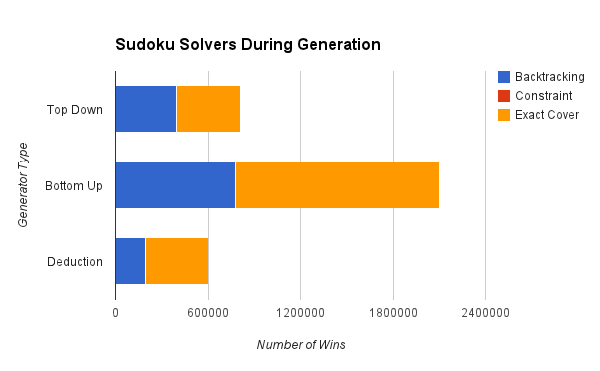
\includegraphics[scale=0.70]{solvers.png}
        \caption{Results of how many times each solver won during each of the generation of sudoku puzzles.}
        \label{fig:solvergen}
    \end{figure}
    As expected, exact cover does win about $60\%$ of the time. However backtracking and constraint propagation are backwards from what was expected
    (note this was \textit{not} an implementation issue!). In fact, constraint propagation won so few times that it doesn't even appear in the graph.
    So why did backtracking do much better than expected? For top down generation, it actually makes sense. Backtracking requires absolutely
    no pre- or post-processing of the data. It just loops through the sudoku, skipping clues already given in the puzzle. During top down generation,
    most of the puzzle is already given, so backtracking has very few calculations to actually do. Meanwhile, constraint propagation and exact
    cover are still pre-processing the puzzle. Backtracking would win while the puzzle is fairly full still, then later exact cover would outperform,
    which is the type of results seen for top down generation.\\
    What about bottom up and deduction generation? Each of those start with an empty sudoku puzzle. Backtracking is still
    a major contender. The difference between the results in the previous section and now is that the formity checks are on puzzles that are
    not well formed, they usually have more than one solution. Each of the solving strategies is a depth first search, so if there are many
    solutions, they would find two similar ones quickly and return that there are multiple solutions. The difference between backtracking
    and the others is again the lack of additional processing. On a near empty sudoku, basically any values you throw into a cell will lead
    to a solution with very little backtracking actually required. So, the same reasoning applies to these generation strategies as top down.
    While exact cover is still pre-processing, backtracking has gotten a head start, and may end up finding two very similar solutions very
    quickly and actually winning.\\
    Constraint propagation didn't do anywhere near as well as expected. This is likely due to the unexpected backtracking results. Backtracking
    does exceptionally well in near full and near empty puzzles while checking for formity. In all other cases, exact cover would simply outperform
    constraint propagation. Given these facts, it makes sense that constraint propagation simply fails to show any results. If one were to redo
    the experiment without using exact cover, my personal estimate is that constraint propagation would take exact cover's position and win
    most of the time against backtracking.
    %\end{Use in Generation}
%\end{Comparison of Solving Strategies}

\subsection{Comparison of Generation Strategies}
As mentioned, $100,000$ sudoku puzzles were generated using each of the three generators. Figure~\ref{fig:generators} shows how each of
the generators performed on average.
\begin{figure}[H]
    \centering
    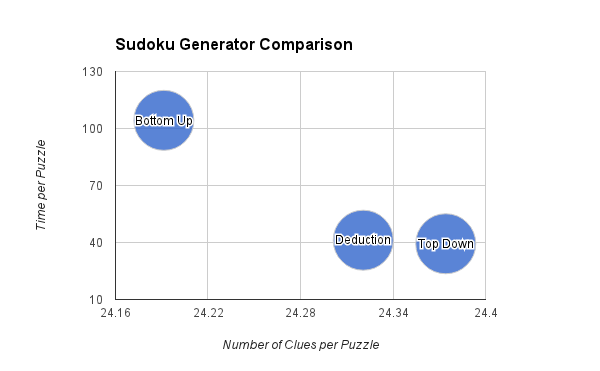
\includegraphics[scale=0.70]{generators.png}
    \caption{Average results of each of the three sudoku puzzle generators.}
    \label{fig:generators}
\end{figure}
Figure~\ref{fig:generators} shows that, on average, the bottom up generation strategy created puzzles with a fewer clues than the other
generation methods, but it also took more time. The average time and number of clues for bottom up generation are skewed however by outliers.
Occasionally, bottom up would "get stuck" on a particular problem. New clues were added, but a unique solution was never obtained,
at least not until a large number of clues was added. This meant that a clue would be added, the solvers would run, no solution was found and the
clue was removed. These types of puzzles took ages to generate, and had many clues compared to all the other bottom up puzzles generated.
Of the $100,000$ generated, about $100$ experienced this problem. These outliers had about double the clues of all the other puzzles, and took
anywhere from $10$ to $100$ times the amount of time to create. Bottom up, even including these outliers, was the most successful generator tested.
It produced puzzles with fewer clues more often than the others, and actually produced the only $19$ clue puzzle found during the testing.\\
Top down and deduction generation seem to be about on par, except for the fact that deduction generation usually produced puzzles with fewer
clues than top down generation in about the same amount of time.\\
Looking back at Figure~\ref{fig:solvergen}, we can see why each generation strategy took as long as they did. Deduction and top down generation
each had to check the formity of about the same number of puzzles - the total width of the bar. Bottom up generation had to check formity about
three times as many puzzles, so it took much longer than the others.
%\end{Comparison of Generation Strategies}

%\end{Results}
